\documentclass[11pt, a4paper]{article}
\usepackage[norsk]{babel}

%For strikethrough
%\usepackage{ulem}

%For landscpe orientation \begin{landscape}...
\usepackage{pdflscape}
\newcommand{\blandscape}{\begin{landscape}}
\newcommand{\elandscape}{\end{landscape}}

%For rotating a figure \begin{sidewaysfigure}...
\usepackage{rotating}
\newcommand{\brotatefig}{\begin{sidewaysfigure}}
\newcommand{\erotatefig}{\end{sidewaysfigure}}


%%\newlength{\cslhangindent}
%\setlength{\cslhangindent}{1.5em}
%\newenvironment{CSLReferences}%
%  {\setlength{\parindent}{0pt}%
%  \everypar{\setlength{\hangindent}{\cslhangindent}}\ignorespaces}%
%  {\par}
%
%To fix CLSreferenses bug
%This will probably have to be updated when using later rmarkdown and or pandoc versions
\newlength{\cslhangindent}
\setlength{\cslhangindent}{3.2em}
\newenvironment{CSLReferences}[2]{
\setlength{\parindent}{0pt}%
  \everypar{\setlength{\hangindent}{\cslhangindent}}\ignorespaces%
  \par}


%For fill text
\usepackage{blindtext}

%For equations
\usepackage{amsmath}
%\savesymbol{medspace}
%\usepackage{txfonts}

%for tables spanning pages
\usepackage{longtable}

%Force floats to appear after text
%\usepackage{flafter}



%For linenumbers

%For references
%\usepackage{natbib} %%Handled by pandoc!
%\bibliographystyle{nina}
\usepackage[hidelinks,
            pdfborder={0 0 0},
            colorlinks = true,
            linkcolor = black,
            urlcolor = darkblue,
            pdfauthor={
                          Skriv in forfatter her
                                       ,~Skriv in forfatter her
                           ,~Skriv in forfatter her
                                       ,~Skriv in siste forfatter her
                         },
            pdftitle={Skriv in titell nivå 1 her},
            pdfsubject={Skriv in titell nivå 2 her},
            pdfkeywords={
                            ,~
                            ,~
                          }]{hyperref}


%For getting total pagecount
\usepackage{lastpage}

%For typesetting of bullet lists
\providecommand{\tightlist}{%
  \setlength{\itemsep}{0pt}\setlength{\parskip}{0pt}}

%To get pdf production date in proper format
\usepackage[norsk]{datetime}
\newdateformat{ninadate}{%
\monthname[\THEMONTH]~ \THEYEAR}

%Set fonts
%Note that we need to suppress ligaturs to mimic standard windows behaviour with Calibri
\usepackage{fontspec}
\defaultfontfeatures{Ligatures={NoRequired, NoCommon, NoContextual}}
\setmainfont{Calibri}
\newfontfamily{\narrow}{Calibri}
\newfontfamily{\narrowbold}{Calibri Bold}
\newfontfamily{\arialnarrow}{Arial Narrow}
\newfontfamily{\arialnarrowbold}{Arial Narrow Bold}
%\restoresymbol{fontspec}{medspace}


%To insert manual hyphens
\usepackage{hyphenat}

%To set caption font
%\usepackage[font=it,labelfont=bf]{caption}
\usepackage[font=it,format=plain,labelfont=bf,justification=justified,singlelinecheck=false,labelsep=period]{caption}

%Modify defaults to restrict the floating of figures
\renewcommand{\topfraction}{.85}
\renewcommand{\bottomfraction}{.7}
\renewcommand{\textfraction}{.15}
\renewcommand{\floatpagefraction}{.66}
\setcounter{topnumber}{3}
\setcounter{bottomnumber}{3}
\setcounter{totalnumber}{4}

%To place table caption above table
\usepackage{float}
\floatstyle{plaintop}
\restylefloat{table}
\setlength{\belowcaptionskip}{3mm}

%To refer to sections, figures and tables
\usepackage{nameref}
\newcommand*{\myref}[1]{\hyperref[{#1}]{\autoref*{#1} \nameref*{#1}}}
%Define own http_links to get underline links
\usepackage{soul}
\setul{.2ex}{.15ex}
\renewcommand*{\href}[2]{\hyperref[#1]{\color{darkblue}\setulcolor{darkblue}\ul{\mbox{#2}}}}
%\renewcommand*{\href}[1]{\hyperref[#1]{\color{darkblue}\setulcolor{darkblue}\ul{\mbox{#1}}}}


%Modify table of contents style
%\usepackage{titlesec}
\usepackage{titletoc}
\setcounter{tocdepth}{4}
%\contentsmargin{2.3em}
\contentsmargin{0em}
%\dottedcontents{section}[2.3em]{\bfseries}{1.3em}{5pt}
\dottedcontents{section}[1.3em]{\bfseries}{1.3em}{5pt}
\dottedcontents{subsection}[4.1em]{}{2.9em}{5pt}
\dottedcontents{subsubsection}[6.6em]{}{2.9em}{5pt}
\dottedcontents{paragraph}[10.2em]{}{3.6em}{5pt} %%too wide dots
\usepackage{setspace}

%To adjust margins and use left justification
\usepackage[a4paper, left=1.5cm,right=3.5cm,top=2cm,bottom=2cm,headheight=1cm]{geometry}
%\usepackage[document]{ragged2e}

%To adjust heading spacings
\usepackage{titlesec}
%To fix bug in titlesec 2.10.1 - that prevented section numbering
\usepackage{etoolbox}
\makeatletter
\patchcmd{\ttlh@hang}{\parindent\z@}{\parindent\z@\leavevmode}{}{}
\patchcmd{\ttlh@hang}{\noindent}{}{}{}
\makeatother
%end fix bug
\titlespacing{\subsection}{0pt}{12pt plus 4pt minus 2pt}{0pt plus 2pt minus 2pt}
\titlespacing{\subsubsection}{0pt}{12pt plus 4pt minus 2pt}{0pt plus 2pt minus 2pt}
\titleformat{\paragraph}
{\normalfont\normalsize\bfseries}{\theparagraph}{1em}{}
\titlespacing*{\paragraph}{0pt}{12pt plus 4pt minus 2pt}{0pt plus 2pt minus 2pt}

\newcommand{\smallspace}{\vspace{3mm}}
%\newcommand{\medspace}{\vspace{5mm}}

%Adjust paragraph indentations
\setlength{\parindent}{0pt}

%To adjust graphics
\usepackage{graphicx}
%\usepackage{epstopdf}

\usepackage{tikz}
\usetikzlibrary{positioning}
\usepackage{xstring}
\usepackage{forloop}


%Modify headers and footers
\usepackage{fancyhdr}
\newsavebox{\myheadbox}
\pagestyle{fancy}
\addtolength{\headheight}{2pt}
\renewcommand{\headrulewidth}{0pt}
\renewcommand{\footrulewidth}{0pt}

%Defines the line in the pagefooter
\newcommand*\ruleline[1]{\par\noindent\raisebox{.4ex}{\makebox[\linewidth]{\hrulefill\hspace{1ex}\raisebox{-.4ex}{#1}\hspace{1ex}\hrulefill}}}

%Define titlepage footer
\usepackage{tikzpagenodes}
\fancypagestyle{titlefooter}{% Define title footer (change to svg logo)
  \fancyhf{}
  \begin{center}
  \vspace{-1.2cm}
  \Large\shadOrange{\narrow{\textbf{www.nina.no}}}
  \vspace{.2cm}
  \end{center}
  \begin{tikzpicture}[remember picture,overlay]
    \node (a) at (-4,-1.68) {};
    \node (b) at (0.37,-8.12) {};
    \coordinate[above=2.5cm of b,xshift=-.6cm]  (legend);
    \coordinate[below=.49cm of a,xshift=3.3cm]  (rapportnr);
    \fill[footgrey] (a) rectangle (b);
    \node[rotate=90] at (legend) {\color{darkgrey}\Huge{\arialnarrowbold{NINA~}\arialnarrow{Rapport}}};
    \node at (rapportnr) {\color{orange}\Huge{\narrowbold{1234}}};
 \end{tikzpicture}
\lfoot{\vspace{1.25cm}\hspace{-1.45cm}
\includegraphics[height=1.6cm]{logo.eps}}
\rfoot{\vspace{2.4cm}\Large\color{darkgrey}{\arialnarrow{Norsk institutt for naturforskning~~~}}}
\begin{tikzpicture}[remember picture,overlay]
  \fill[footgrey]
    (current page.south west)
    rectangle
  (current page.east|-current page footer area.south east);
  \end{tikzpicture}
}

 \usepackage{tikzpagenodes}


% one way of including bg-pic
% \usepackage{eso-pic}
% \newcommand\BackgroundPic{%
% \put(0,0){%
% \parbox[b][\paperheight]{\paperwidth}{%
% \vfill
% \centering
% \includegraphics[width=\paperwidth,height=\paperheight,%
% keepaspectratio]{title_page_bg.png}%
% \vfill
% }}}

%Define endpage footer
\fancypagestyle{endfooter}{% Define endpage footer (change to svg logo)

  \fancyhf{}
  \fancyfootoffset[R]{0cm}
  \begin{center}
    \vspace{-1.2cm}
    \Large\shadOrange{\narrow{\textbf{www.nina.no}}}

 \begin{tikzpicture}[remember picture,overlay]
 \node (a) at (11.05, 4.3) {};
 \node (b) at (15,-2.1) {};
 \coordinate[above=2.5cm of b,xshift=-3cm]  (legend);
 \coordinate[below=.5cm of a,xshift=1cm]  (rapportnr);
 \fill[footgrey] (a) rectangle (b);
 \node[rotate=90] at (legend) {\color{darkgrey}\Huge{\arialnarrowbold{NINA~}\arialnarrow{Rapport}}};
 \node at (rapportnr) {\color{orange}\huge{\narrowbold{1234}}};
\end{tikzpicture}
    \begin{minipage}{0.386\linewidth}
    {\begin{flushleft}\color{darkgrey}\vspace{1.2cm}\large\narrow\em{\textbf{Norsk institutt for naturforskning, NINA,} er en uavhengig stiftelse som forsker på natur og samspillet natursammfunn.

    \bigskip
    NINA ble etablert i 1988. Hovedkontoret er i Trondheim, med avdelingskontorer i Tromsø, Lillehammer, Bergen og Oslo. I tillegg driver NINA Sæterfjellet avlsstasjon for fjellrev på Oppdal, og forskningsstasjonen for vill laksefisk på Ims i Rogaland.

    \bigskip
    NINAs virksomhet omfatter både forskning og utredning, miljøoveråking, rådgivning og evaluering. NINA har stor bredde i kompetanse og erfaring med både naturvitere og samfunnsvitere i staben. Vi har kunnskap om artene, naturtypene, sammfunnets bruk av naturen og sammenhenger med de store drivkreftene i naturen.} \end{flushleft}}
    \end{minipage}
    \vspace{3cm}
    \vfill{}{\normalsize{ISSN: 1504-3312 \\
  ISBN: 978-82-426-1234-5}}
  \end{center}
  \lfoot{\color{darkgrey}\vspace{0.5cm}\Large\narrow{\textbf{Norsk institutt for naturforskning}}\\
\begingroup
\narrow
\normalsize NINA Hovedkontor\\
Postadresse: Postboks 5685 Torgarden, 7485 Trondheim\\
Besøks-/leveringsadresse: Høgskoleringen 9, 7034 Trondheim\\
Telefon: 73 80 14 00, Telefaks: 73 80 14 01\\
E-post: firmapost@nina.no\\
Organisasjonsnummer 9500 37 687\\
http://www.nina.no
\endgroup}
  % \rfoot{\vspace{2cm}\hspace{-3cm}
\includegraphics[height=1.6cm]{logo.eps}\\
  % \Large\darkGrey{\narrow{Samarbeid og kunnskap for framtidas miljøløsninger}}
  % }
  \rfoot{\vspace{2.3cm}\savebox{\myheadbox}{\Large\darkGrey{\narrow{Samarbeid og kunnskap for framtidas miljøløsninger}}}\makebox[\wd\myheadbox][c]{
\includegraphics[height=1.6cm]{logo.eps}}\\\usebox{\myheadbox}}

    \begin{tikzpicture}[remember picture,overlay]
  \fill[footgrey]
    (current page.south west)
    %(current page.west|-current page footer area.north west)
    rectangle
  (current page.east|-current page footer area.north east);
  %(current page text area.south west);
  \end{tikzpicture}

%  \tikz[remember picture,overlay] {%
%  \draw [blue,line width=2mm]
%  (current page.south west)
%  rectangle
%  (current page.north east)
%  ;
%  \draw [green]
%  (current page text area.south west)
%  rectangle
%  (current page text area.north east)
%  ;
%  \draw [yellow]
%  (current page marginpar area.south west)
%  rectangle
%  (current page marginpar area.north east)
%  ;
%  \draw [red]
%  (current page header area.south west)
%  rectangle
%  (current page header area.north east)
%  ;
%  \draw [orange]
%  (current page footer area.south west)
% rectangle
%  (current page footer area.north east)
%  ;
%  }%

}

%Make sure it always produce even numbered document (adding empty page if necessary)
\usepackage{scrextend}
\newcommand{\OpenNewPageIfNeeded}{%
  \Ifthispageodd{\fancyhf{}\newgeometry{bottom=6.6cm, top=2cm, left=1.5cm, right=1.5cm, headsep=0cm, footskip=0.5cm}\null\clearpage~\pagestyle{endfooter}
  }{\fancyhf{}\newgeometry{bottom=6.6cm, top=2cm, left=1.5cm, right=1.5cm, headsep=0cm, footskip=0.5cm}\null\pagestyle{endfooter}}
}
\AtEndDocument{\OpenNewPageIfNeeded}


\usepackage{color}
\usepackage{fancyvrb}
\newcommand{\VerbBar}{|}
\newcommand{\VERB}{\Verb[commandchars=\\\{\}]}
\DefineVerbatimEnvironment{Highlighting}{Verbatim}{commandchars=\\\{\}}
% Add ',fontsize=\small' for more characters per line
\usepackage{framed}
\definecolor{shadecolor}{RGB}{241,243,245}
\newenvironment{Shaded}{\begin{snugshade}}{\end{snugshade}}
\newcommand{\AlertTok}[1]{\textcolor[rgb]{0.68,0.00,0.00}{#1}}
\newcommand{\AnnotationTok}[1]{\textcolor[rgb]{0.37,0.37,0.37}{#1}}
\newcommand{\AttributeTok}[1]{\textcolor[rgb]{0.40,0.45,0.13}{#1}}
\newcommand{\BaseNTok}[1]{\textcolor[rgb]{0.68,0.00,0.00}{#1}}
\newcommand{\BuiltInTok}[1]{\textcolor[rgb]{0.00,0.23,0.31}{#1}}
\newcommand{\CharTok}[1]{\textcolor[rgb]{0.13,0.47,0.30}{#1}}
\newcommand{\CommentTok}[1]{\textcolor[rgb]{0.37,0.37,0.37}{#1}}
\newcommand{\CommentVarTok}[1]{\textcolor[rgb]{0.37,0.37,0.37}{\textit{#1}}}
\newcommand{\ConstantTok}[1]{\textcolor[rgb]{0.56,0.35,0.01}{#1}}
\newcommand{\ControlFlowTok}[1]{\textcolor[rgb]{0.00,0.23,0.31}{#1}}
\newcommand{\DataTypeTok}[1]{\textcolor[rgb]{0.68,0.00,0.00}{#1}}
\newcommand{\DecValTok}[1]{\textcolor[rgb]{0.68,0.00,0.00}{#1}}
\newcommand{\DocumentationTok}[1]{\textcolor[rgb]{0.37,0.37,0.37}{\textit{#1}}}
\newcommand{\ErrorTok}[1]{\textcolor[rgb]{0.68,0.00,0.00}{#1}}
\newcommand{\ExtensionTok}[1]{\textcolor[rgb]{0.00,0.23,0.31}{#1}}
\newcommand{\FloatTok}[1]{\textcolor[rgb]{0.68,0.00,0.00}{#1}}
\newcommand{\FunctionTok}[1]{\textcolor[rgb]{0.28,0.35,0.67}{#1}}
\newcommand{\ImportTok}[1]{\textcolor[rgb]{0.00,0.46,0.62}{#1}}
\newcommand{\InformationTok}[1]{\textcolor[rgb]{0.37,0.37,0.37}{#1}}
\newcommand{\KeywordTok}[1]{\textcolor[rgb]{0.00,0.23,0.31}{#1}}
\newcommand{\NormalTok}[1]{\textcolor[rgb]{0.00,0.23,0.31}{#1}}
\newcommand{\OperatorTok}[1]{\textcolor[rgb]{0.37,0.37,0.37}{#1}}
\newcommand{\OtherTok}[1]{\textcolor[rgb]{0.00,0.23,0.31}{#1}}
\newcommand{\PreprocessorTok}[1]{\textcolor[rgb]{0.68,0.00,0.00}{#1}}
\newcommand{\RegionMarkerTok}[1]{\textcolor[rgb]{0.00,0.23,0.31}{#1}}
\newcommand{\SpecialCharTok}[1]{\textcolor[rgb]{0.37,0.37,0.37}{#1}}
\newcommand{\SpecialStringTok}[1]{\textcolor[rgb]{0.13,0.47,0.30}{#1}}
\newcommand{\StringTok}[1]{\textcolor[rgb]{0.13,0.47,0.30}{#1}}
\newcommand{\VariableTok}[1]{\textcolor[rgb]{0.07,0.07,0.07}{#1}}
\newcommand{\VerbatimStringTok}[1]{\textcolor[rgb]{0.13,0.47,0.30}{#1}}
\newcommand{\WarningTok}[1]{\textcolor[rgb]{0.37,0.37,0.37}{\textit{#1}}}
%Define custom code background shading
\definecolor{shadecolor}{RGB}{238,238,238}


%Set up custom colors
\usepackage{xcolor}
\usepackage{blindtext}
\definecolor{darkOrange}{RGB}{245,127, 0}
\definecolor{lightOrange}{RGB}{219,140, 68}
\definecolor{ashgrey}{RGB}{128, 128, 128}
\definecolor{darkgrey}{RGB}{66, 85, 99}
\definecolor{footgrey}{RGB}{212, 215, 221}
\definecolor{darkblue}{RGB}{0, 79, 113}

\newcommand{\shadOrange}[1]{\textcolor{lightOrange}{#1}}
\newcommand{\orange}[1]{\textcolor{darkOrange}{#1}}
\newcommand{\lightGrey}[1]{\textcolor{ashgrey}{#1}}
\newcommand{\darkGrey}[1]{\textcolor{darkgrey}{#1}}

\begin{document}
%\AddToShipoutPicture*{\BackgroundPic}

\newgeometry{bottom=6cm, top=4.6cm, left=3.48cm, right=1.5cm}

\begin{titlepage}
%Testing out title page bg-pic
\thispagestyle{titlefooter}

%Testing out tikz title page bg-pic
% \begin{tikzpicture}[remember picture,overlay, anchor=south west]
%   \node at (current page.south west){\includegraphics[width=\paperwidth,height=\paperheight,%
%  keepaspectratio]{title_page_bg.png}};
% \end{tikzpicture}

\huge{Skriv in titell nivå 1 her} \par\vspace{.3cm}
\LARGE{Skriv in titell nivå 2 her} \par\vspace{.6cm}
\hspace{0cm}\Large{Skriv in forfatter her},
\hspace{-2mm}~\Large{Skriv in forfatter her},
\hspace{-2mm}~\Large{Skriv in forfatter her},
\hspace{-2mm}~\Large{Skriv in siste forfatter her}

\begin{tikzpicture}[remember picture,overlay, anchor=south west]
  \node at ([yshift=4.77cm,xshift=-0.24cm]current page.south west){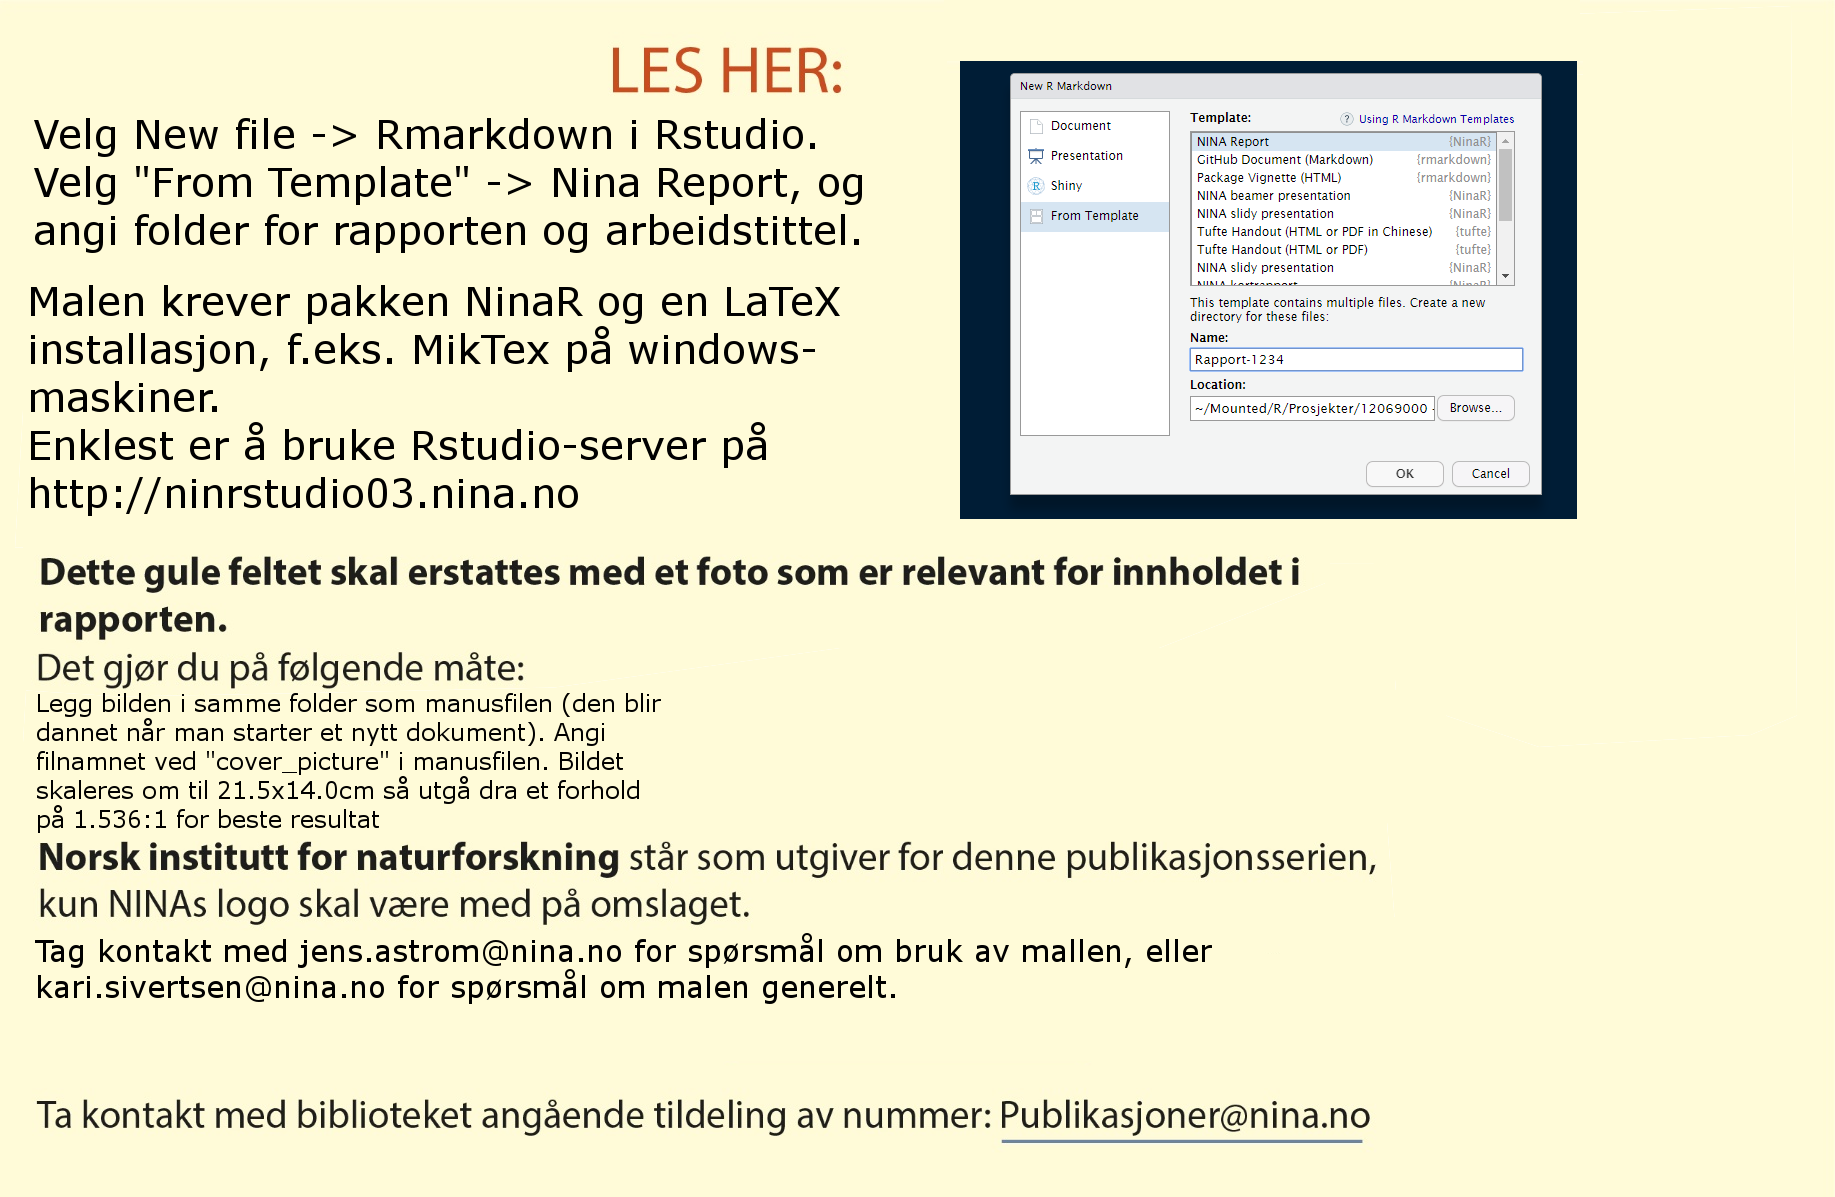
\includegraphics[width=21.35cm, height=13.9cm]{coverPicture.png}};
 \end{tikzpicture}
\restoregeometry
\end{titlepage}
\newgeometry{bottom=3cm, top=3cm, left=2.68cm, right=2.68cm}
%Second page
\cfoot{}

\section*{\narrow{NINAs publikasjoner}}
\hspace{1ex}

\subsection*{\small{NINA Rapport}}
{\normalsize Dette er NINAs ordinære rapportering til oppdragsgiver etter gjennomført forsknings\hyp{}, overvåkings\hyp{} eller utredningsarbeid. I tillegg vil serien favne mye av instituttets øvrige rapportering, for eksempel fra seminarer og konferanser, resultater av eget forsknings\hyp{} og utredningsarbeid og litteraturstudier. NINA Rapport kan også utgis på engelsk, som NINA Report.
}

\subsection*{\small{NINA Temahefte}}
{\normalsize Heftene utarbeides etter behov og serien favner svært vidt; fra systematiske bestemmelsesnøkler til informasjon om viktige problemstillinger i samfunnet. Heftene har vanligvis en populærvitenskapelig form med vekt på illustrasjoner. NINA Temahefte kan også utgis på engelsk, som NINA Special Report.}

\subsection*{\small{NINA Fakta}}
{\normalsize Faktaarkene har som mål å gjøre NINAs forskningsresultater raskt og enkelt tilgjengelig for et større
publikum. Faktaarkene gir en kort framstilling av noen av våre viktigste forskningstema.}

\subsection*{\small{Annen publisering}}
{\normalsize I tillegg til rapporteringen i NINAs egne serier publiserer instituttets ansatte en stor del av sine forsk- ningsresultater i internasjonale vitenskapelige journaler og i populærfaglige bøker og tidsskrifter.}
\clearpage
\newgeometry{bottom=3cm, top=3cm, left=2.68cm, right=2.68cm}
%Page 3
\setcounter{page}{1}
\fancyfoot[C]{
\newgeometry{bottom=3cm, top=3cm, left=2.68cm, right=2cm}
\vspace{-0.5cm}\hfill\Large{\narrowbold{Norsk institutt for naturforskning}}}
\vspace{2cm}

\huge{Skriv in titell nivå 1 her} \par\vspace{.5cm}
\LARGE{Skriv in titell nivå 2 her} \par\vspace{1cm}
\hspace{0cm}\LARGE{Skriv in forfatter her} \par
\LARGE{Skriv in forfatter her} \par
\LARGE{Skriv in forfatter her} \par
\LARGE{Skriv in siste forfatter her} \par

\clearpage
\newgeometry{bottom=2.5cm, top=2.5cm, left=2.5cm, right=2.5cm}
%Page 4
\fancyhf{}
\pagestyle{fancy}
\fancyfoot[c]{\ruleline{\thepage}}
\fancyhead[c]{\ruleline{\tiny{NINA Rapport 1234}}}
% To count also the first page (for new template)
\addtocounter{page}{1}

\normalsize
\newgeometry{bottom=3cm, top=2.6cm, left=2.82cm, right=6.2cm}
\small{Brum, O., Robin, K. 2016. En veldig bra
titel.}~NINA Rapport 1234. Norsk institutt for naturforskning. \par \href{http://hdl.handle.net/11250/fås
av bibliotek}{http://hdl.handle.net/11250/fås av
bibliotek} \par \smallspace
Trondheim, \ninadate\today \par \smallspace
ISSN: 1504-3312 \par
ISBN: 978-82-426-1234-5 \par  \smallspace
{\scriptsize{RETTIGHETSHAVER}} \par
© Norsk institutt for naturforskning  \par
Denne rapporten er lisensiert under Creative Commons Navngivelse 4.0 \par
Internasjonal lisens: \href{https://creativecommons.org/licenses/by/4.0/}{Creative Commons — Attribution 4.0 International — CC BY 4.0}\par \smallspace
{\scriptsize{TILGJENGELIGHET}} \par
Åpen \par \smallspace
{\scriptsize{PUBLISERINGSTYPE}} \par
Digitalt dokument (pdf) \par \smallspace
{\scriptsize{KVALITETSSIKRET AV}} \par
xx \par \smallspace
{\scriptsize{ANSVARLIG SIGNATUR}} \par
Forskningssjef Forskningssjef {[}fylles ut av forskningssjefen{]}
(sign.) \par \smallspace
{\scriptsize{OPPDRAGSGIVER(E)/BIDRAGSYTER(E)}} \par
xx \par \smallspace
{\scriptsize{OPPDRAGSGIVERS REFERANSE}} \par
xx \par \smallspace
{\scriptsize{KONTAKTPERSON(ER) HOS OPPDRAGSGIVER/BIDRAGSYTER}} \par
xx \par \smallspace
{\scriptsize{FORSIDEBILDE}} \par
Forsidebildetekst~ \copyright~ Fotografnavn \par \smallspace
{\scriptsize{NØKKELORD}} \par\smallskip
\small{\hyp{} } \par
\small{\hyp{} } \par
\vspace{5mm}
{\scriptsize{KEY WORDS}} \par\smallskip
\small{\hyp{} } \par

\vfill
%\noindent


\begin{minipage}{\linewidth}
\scriptsize{KONTAKTOPPLYSNINGER} \par\smallspace
\scriptsize
\leavevmode\hbox to \linewidth{%
\hspace{-.25cm}
\begin{tabular}[t]{l@{}}
\textbf{NINA hovedkontor} \\
Postboks 5685 Torgarden\\
7485 Trondheim\\
Telefon: 73 80 14 00
\end{tabular}
\hfill
\begin{tabular}[t]{l@{}}
\textbf{NINA Oslo} \\
Sognsveien 68 \\
0855 Oslo \\
Telefon: 73 80 14 00
\end{tabular}%
\hfill
\begin{tabular}[t]{l@{}}
\textbf{NINA Tromsø} \\
Postboks 6606 Langnes \\
9296 Tromsø \\
Telefon: 77 75 04 00
\end{tabular}%
\hfill
\begin{tabular}[t]{l@{}}
\textbf{NINA Lillehammer} \\
Vormstuguvegen 40 \\
2624 Lillehammer \\
Telefon: 73 80 14 00
\end{tabular}%
\begin{tabular}[t]{l@{}}
\textbf{NINA Bergen} \\
Thormøhlensgate 55 \\
5006 Bergen \\
Telefon: 73 80 14 00
\end{tabular}%
}
\par\vspace{3mm}
www.nina.no
\vspace{-4mm}
\end{minipage}

\clearpage
\setcounter{secnumdepth}{0}
\newgeometry{bottom=3cm, top=3cm, left=2.68cm, right=2.68cm}
\section{Sammendrag}
\normalsize{Brum, O., Robin, K. 2016. En veldig bra
titel.} NINA Rapport 1234. Norsk institutt for naturforskning. \par\href{http://hdl.handle.net/11250/fås
av bibliotek}{http://hdl.handle.net/11250/fås av bibliotek} \par
\vspace{0.5cm}
\normalsize{
Tekst inn her, et kort resymé av innholdet.
\textbf{Maksimalt 4000 tegn inkl. ordmellomrom. Dette er maxgrense i sammendragsfeltet i CRIStin, og dersom sammendraget er lengre kommer det ikke med her.}
Teksten i sammendraget er søkbar i databaser og på nett, og er viktig
for at rapporten skal fanges opp ved søk.\\
\strut \\
Seksjoner og tomme rader mellom dem er litt tricky å få til i
YAML-avsnittet, men det kan gjøres slik. Tomme rader i forordet kan også
lages på samme måte.} \\

\vspace{1cm}
\small
Skriv in forfatter her, Author adress, for.efternavn@nina.no  \par
Skriv in forfatter her, Author adress, for.efternavn@nina.no  \par
Skriv in forfatter her, Author adress, for.efternavn@nina.no  \par
Skriv in siste forfatter her, Author adress, for.efternavn@nina.no  \par
\normalsize
\clearpage

\setcounter{secnumdepth}{0}
\section{Abstract}
\small{the Poo, W., Robin, C. 2016. A very good
title.} NINA Rapport 1234. Norsk institutt for naturforskning. \par\href{http://hdl.handle.net/11250/fås
av bibliotek}{http://hdl.handle.net/11250/fås av bibliotek}\par
\vspace{0.5cm}
\normalsize{
Tekst inn her, et kort resymé av innholdet.
\textbf{Maksimalt 4000 tegn inkl. ordmellomrom. Dette er maxgrense i sammendragsfeltet i CRIStin, og dersom sammendraget er lengre kommer det ikke med her.}
Teksten i sammendraget er søkbar i databaser og på nett, og er viktig
for at rapporten skal fanges opp ved søk.} \\

\vspace{1cm}
\small
Skriv in forfatter her, Author adress, for.efternavn@nina.no  \par
Skriv in forfatter her, Author adress, for.efternavn@nina.no  \par
Skriv in forfatter her, Author adress, for.efternavn@nina.no  \par
Skriv in siste forfatter her, Author adress, for.efternavn@nina.no  \par
\normalsize
\clearpage


\doublespacing
\tableofcontents
\addcontentsline{toc}{section}{Innhold}
\singlespacing
\clearpage

\section{Forord}

\normalsize
Forord inn her\par
\medskip
Stedforord, \par
\medskip
Prosjektleder



\clearpage
\setcounter{secnumdepth}{4}
\setlength{\parskip}{6pt}

\hypertarget{inl}{%
\section{Innledning}\label{inl}}

Dette er et eksempel på en NINA Rapport produsert fra
statistikkprogrammet R, gjennom pakken \texttt{NinaR} (Åström 2016). Den
kan med fordel brukes da rapporten har stort innhold av R-skript.
Bortsett fra seksjonene med kod er mallen tenkt å etterligne NINA sin
standardmalle for rapporter. Malen brukes på samme måte som andre maller
i pakken \texttt{Rmarkdown} (Allaire, Cheng, et al. 2016) og
\texttt{rticles} (Allaire, R Foundation, et al. 2016) (se
http://rmarkdown.rstudio.com/). Rstudio er særskilt tilpasset til
\texttt{rmarkdown}, men malen kan også brukes direkte i R (også via
terminalen/Command Prompt). I Rstudio bruker man enklest knappen
``Knit'', men rapporten kan også genereres med kommandoen
\texttt{rmarkdown::render("din\_rapport.Rmd")}.

\hypertarget{fremgangsmuxe5te}{%
\subsection{Fremgangsmåte}\label{fremgangsmuxe5te}}

\emph{For å bruke malen trengs:}

\begin{itemize}
\tightlist
\item
  R
\item
  NinaR (se http://www.github.com/NINAnor/NinaR)
\item
  En Tex-installasjon

  \begin{itemize}
  \tightlist
  \item
    For Windows, se http://miktex.org/
  \item
    For Mac, se http://tug.org/mactex/
  \item
    For Linux, installere tex-live
  \end{itemize}
\end{itemize}

Den enkleste måten er å bruke rstudio-servene http://rstudio.nina.no,
der alt er (bør være) installert.

Når R-pakken \texttt{NinaR} er installert, finner man malen i Rstudio
gjennom
\texttt{File\ -\textgreater{}\ New\ File\ -\textgreater{}\ R\ Markdown\ -\textgreater{}\ From\ templates}.
Alternativt kan en mal produseres gjennom
\texttt{rmarkdown::draft("title",\ template="nina\_rapport",\ package="NinaR")}.

Høyst oppe i malen (vises ikke i PDFen) finns en såkalt ``YAML-seksjon''
der diverse obligatoriske ting skal skrives inn. En lukket PDF kan lages
gjennom å skrive ``yes'' etter secure\_pdf. Radnummer til review
produseres gjennom \texttt{line\_numbering:\ yes}. Selv-referansen på
side 3 skrives manuelt inn i ved \texttt{self-ref:} i YAML-avsnittet.

Referanser kan inkluderes på to måter. Vi kan for eksempel referere til
Pedersen et al. (2016) i teksten, eller så her (Pedersen et al. 2016).
Stilen for referansene er avhengig at man klasser dem som rett type, for
eksempel som artikel (Adams 1993).

\hypertarget{test-sub-sub-heading}{%
\subsubsection{Test sub sub heading}\label{test-sub-sub-heading}}

For å lage en ``pagebreak'', for eksempel mellom ulike kapittel, skriv
\texttt{\textbackslash{}newpage}. \texttt{\textbackslash{}clearpage}
fungerer på lignende måte, men da tvinger man frem en plassering av alle
bilder til nå, og da kan de ofte havne på en egen side. Prøv deg frem.

\hypertarget{en-til-sub-sub-heading}{%
\subsubsection{En til sub sub heading}\label{en-til-sub-sub-heading}}

Denne male er fortsatt ikke perfekt, men har blitt brukt for et prosjekt
til Miljødirektoratet og godkjent av biblioteket. Spørsmål og
synspunkter kan sendes til Jens Åström.

Det kan gå kjappere å skrive rapporter i dette format, men det gjenstår
ofte noen småfiks med formateringer på slutten. Plassering av bilder kan
til hvis grad styres gjennom å endre på størrelsen til dem (f.eks.
out.width eller fig.width), eller gjennom å overstyre plasseringen
(f.eks. fig.pos = ``!hb''). Men alt er ikke mulig å styre helt så
foreløpig må man akseptere noen plasseringer.

\paragraph{Prøver meg på en sub sub sub heading}

Obs at 4-nivåseksjoner må skrives med
\texttt{\textbackslash{}paragraph\{titell\}}!

\newpage

\hypertarget{res}{%
\section{Resultater}\label{res}}

R-kod kan legges til på vanlig vis. Fargemønstret kan endres gjennom
\texttt{highlight:\ xxx} Yaml-avsnittet i starten på dokumentet.

\begin{Shaded}
\begin{Highlighting}[]
\CommentTok{\# Slik vises kode{-}kommentarer}

\NormalTok{x }\OtherTok{\textless{}{-}} \DecValTok{1}\SpecialCharTok{:}\DecValTok{10} \SpecialCharTok{*} \FloatTok{0.5} \SpecialCharTok{+} \FunctionTok{rnorm}\NormalTok{(}\DecValTok{10}\NormalTok{, }\AttributeTok{mean =} \DecValTok{1}\NormalTok{, }\AttributeTok{sd =} \DecValTok{2}\NormalTok{)}
\NormalTok{y }\OtherTok{\textless{}{-}} \DecValTok{1}\SpecialCharTok{:}\DecValTok{10}
\end{Highlighting}
\end{Shaded}

Tabeller fra R kan lages gjennom pakken \texttt{xtable}. Her er et
eksempel på output fra en enkel modell. Man kan også referere til en
tabell, for eksempel referer jeg nå til tabell \ref{tab1}.

\begin{Shaded}
\begin{Highlighting}[]
\NormalTok{mod1 }\OtherTok{\textless{}{-}} \FunctionTok{glm}\NormalTok{(y }\SpecialCharTok{\textasciitilde{}}\NormalTok{ x)}
\FunctionTok{print}\NormalTok{(}\FunctionTok{xtable}\NormalTok{(}\FunctionTok{round}\NormalTok{(}\FunctionTok{summary}\NormalTok{(mod1)}\SpecialCharTok{$}\NormalTok{coefficients, }\DecValTok{3}\NormalTok{),}
    \AttributeTok{caption =} \StringTok{"Tabell laget med xtable }\SpecialCharTok{\textbackslash{}\textbackslash{}}\StringTok{label\{tab1\}"}\NormalTok{))}
\end{Highlighting}
\end{Shaded}

\begin{table}[ht]
\centering
\begin{tabular}{rrrr}
  \hline
Estimate & Std. Error & t value & Pr($>$$|$t$|$) \\ 
  \hline
3.48 & 1.56 & 2.23 & 0.06 \\ 
  0.50 & 0.32 & 1.57 & 0.16 \\ 
   \hline
\end{tabular}
\caption{Tabell laget med xtable \label{tab1}} 
\end{table}

Figurer fungerer på vanlig vis. Figurtekst lages hvis
\texttt{fig\_caption:\ yes} er angitt i Yaml-avsnittet. Figurteksten
legges til som i eksemplet nedenfor. Hvis man angir
\texttt{\textbackslash{}\textbackslash{}label\{\}} i figurteksten kan
man også referere til figuren. Figur \ref{xy_plot} viser et eksempel på
bruk av NINAs logofarger via funksjonen \texttt{NinaR::NinaPalette}.

\begin{Shaded}
\begin{Highlighting}[]
\NormalTok{plot.mat }\OtherTok{\textless{}{-}} \FunctionTok{matrix}\NormalTok{(}\FunctionTok{rnorm}\NormalTok{(}\DecValTok{25}\NormalTok{, }\DecValTok{40}\NormalTok{, }\AttributeTok{sd =} \DecValTok{10}\NormalTok{), }\AttributeTok{ncol =} \DecValTok{5}\NormalTok{,}
    \AttributeTok{dimnames =} \FunctionTok{list}\NormalTok{(}\FunctionTok{c}\NormalTok{(}\StringTok{"Sportsfisker"}\NormalTok{, }\StringTok{"Elveeier"}\NormalTok{, }\StringTok{"Oppleid"}\NormalTok{,}
        \StringTok{"Fisket"}\NormalTok{, }\StringTok{"Poseidon"}\NormalTok{), }\FunctionTok{c}\NormalTok{(}\StringTok{"Lakselus"}\NormalTok{, }\StringTok{"Utsetting"}\NormalTok{,}
        \StringTok{" Strengere restriksjoner"}\NormalTok{, }\StringTok{"Fysiske tiltak"}\NormalTok{,}
        \StringTok{"Flaks"}\NormalTok{)))}

\NormalTok{plot.mat }\OtherTok{\textless{}{-}}\NormalTok{ tibble}\SpecialCharTok{::}\FunctionTok{tibble}\NormalTok{(}\AttributeTok{Verdi =} \FunctionTok{rnorm}\NormalTok{(}\AttributeTok{n =} \DecValTok{25}\NormalTok{, }\AttributeTok{mean =} \DecValTok{40}\NormalTok{,}
    \AttributeTok{sd =} \DecValTok{10}\NormalTok{), Prøvetyper }\OtherTok{=} \FunctionTok{rep}\NormalTok{(}\FunctionTok{c}\NormalTok{(}\StringTok{"Type\_1"}\NormalTok{, }\StringTok{"Type\_2"}\NormalTok{,}
    \StringTok{"Type\_3"}\NormalTok{, }\StringTok{"Type\_4"}\NormalTok{, }\StringTok{"Type\_5"}\NormalTok{), }\AttributeTok{each =} \DecValTok{5}\NormalTok{), }\AttributeTok{Kategori =} \FunctionTok{rep}\NormalTok{(}\FunctionTok{c}\NormalTok{(}\StringTok{"Lengde"}\NormalTok{,}
    \StringTok{"Høyde"}\NormalTok{, }\StringTok{"Dybde"}\NormalTok{, }\StringTok{"Vekt"}\NormalTok{, }\StringTok{"Kvalitet"}\NormalTok{), }\AttributeTok{times =} \DecValTok{5}\NormalTok{))}

\FunctionTok{ggplot}\NormalTok{(plot.mat) }\SpecialCharTok{+} \FunctionTok{geom\_bar}\NormalTok{(}\FunctionTok{aes}\NormalTok{(}\AttributeTok{x =}\NormalTok{ Verdi, }\AttributeTok{y =}\NormalTok{ Prøvetyper,}
    \AttributeTok{fill =}\NormalTok{ Kategori), }\AttributeTok{stat =} \StringTok{"identity"}\NormalTok{, }\AttributeTok{position =} \StringTok{"dodge"}\NormalTok{) }\SpecialCharTok{+}
    \FunctionTok{scale\_fill\_nina}\NormalTok{()}
\end{Highlighting}
\end{Shaded}

\begin{figure}[H]

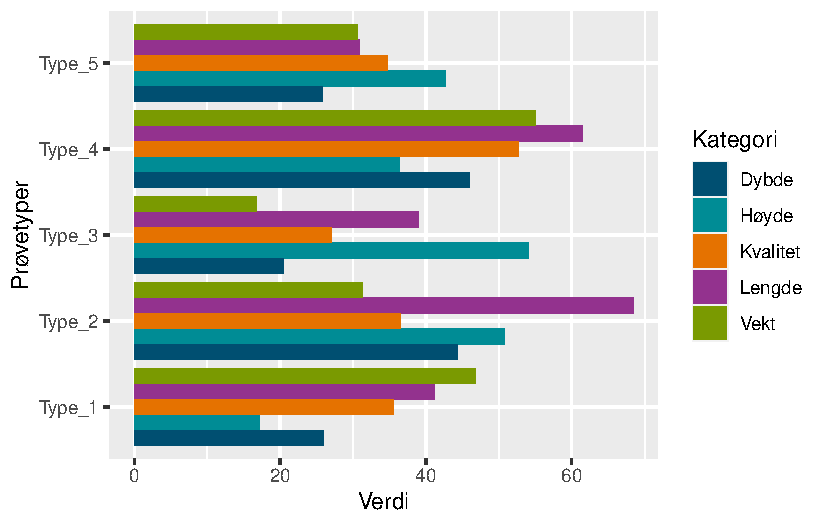
\includegraphics{quarto_ninareport_files/figure-pdf/test-chunk3-1.pdf} \hfill{}

\caption{Ett exempel med NINAs fargepalett generert fra R.
\label{xy_plot}}

\end{figure}

Eksisterende bilder kan også legges til gjennom vanlig markdown syntax.
Disse blir sentrerte. Noter at eps-filer angis uten filendelse.

\begin{figure}

{\centering 
\includegraphics{logo.eps}

}

\caption{Nina-logoen, som eksempel på inkludering av et bilde.
\label{logoen}}

\end{figure}

Hvis man trenger flere muligheter for definisjon av størrelse og
plassering på en ferdig bilde, kan man også inkludere den med
``include\_graphics''.

\begin{figure}


\includegraphics[width=10cm,height=\textheight]{logo.eps} \hfill{}

\caption{NINA-logoen i større format \label{logo_stor}}

\end{figure}

Vi kan også referere til bilder, for eksempel til figur \ref{logoen},
som er inkludert i mallen. Notere at man må ha to
\texttt{\textbackslash{}\textbackslash{}} for figurer laget i R men en
\texttt{\textbackslash{}} for ``eksterne'' bilder. Man kan referere til
seksjoner ved å angi en referanse i headingen \texttt{\{\#seksjon\}}. Se
dette eksempel for å referere til innledningen i kapittel \ref{inl}.

\clearpage

\hypertarget{references}{%
\section{Referanser}\label{references}}

\setlength{\parindent}{-0.2in}
\setlength{\parskip}{8pt}

\noindent

\hypertarget{refs}{}
\begin{CSLReferences}{1}{0}
\leavevmode\vadjust pre{\hypertarget{ref-article}{}}%
Adams, Peter. 1993. {``The Title of the Work.''} \emph{The Name of the
Journal} 4 (2): 201--13.

\leavevmode\vadjust pre{\hypertarget{ref-rmarkdown}{}}%
Allaire, JJ, Joe Cheng, Yihui Xie, Jonathan McPherson, Winston Chang,
Jeff Allen, Hadley Wickham, Aron Atkins, and Rob Hyndman. 2016.
\emph{Rmarkdown: Dynamic Documents for r}.
\url{http://CRAN.R-project.org/package=rmarkdown}.

\leavevmode\vadjust pre{\hypertarget{ref-rticles}{}}%
Allaire, JJ, R Foundation, Hadley Wickham, Journal of Statistical
Software, Yihui Xie, Ramnath Vaidyanathan, Assocation for Computing
Machinery, et al. 2016. \emph{Rticles: Article Formats for r Markdown}.

\leavevmode\vadjust pre{\hypertarget{ref-NinaR}{}}%
Åström, J. 2016. \emph{NinaR: Document Templates and Functions for
NINA}. \url{http://github.com/NINAnor/NinaR}.

\leavevmode\vadjust pre{\hypertarget{ref-Pedersen2016}{}}%
Pedersen, Hans Christian, Arne Follestad, Jan Ove Gjershaug, and Erlend
Birkeland Nilsen. 2016. {``Statusoversikt for Jaktbart Småvilt.''} NINA
rapport 1178. Trondheim: Norsk institutt for naturforskning.
\url{http://www.nina.no/archive/nina/PppBasePdf/rapport/2016/1178.pdf}.

\end{CSLReferences}


%\clearpage
%\fancyhf{}
%\newgeometry{a4paper, bottom=8cm, top=2cm, left=1.5cm, right=1.5cm}
%\pagestyle{endfooter}

\end{document}
